\chapter{TOWARDS HIGH DIMENSION}
\label{chap:highdor}
\graphicspath{{HiDof/HiDofFigs/EPS/}{HiDof/HiDofFigs/}}
\section{Introduction}
In the previous chapters, motions are dynamically synthesized for characters with simplified dynamics.
A question arises whether the  motor invariant theory(\moit) is applicable to characters with higher degrees of freedom.
For walk and stance examples, high degree system will incorporate the motions of the torso and arm.
Also for the snakes and fishes, synthesise motion for the flexible vertebrate may also be a challenge.
\moit provides a different perspective, and some of the challenge can be solved in a very different manner.



Redundant {\dof} is the key challenge in motion synthesis.
From the theoretical perspective of \moit, redundant {\dof s don't increase the computational burden exponentially.
\moit explores the natural dynamics of the body and the redundant {\dof} can move passively.
For the passive walker, all the \dof s are uncontrolled, increased {\dof} s will not increase controller burden.
The computational burden of neural oscillator remains constant during increase of {\dof} s in dynamic model.
The computational burden for controlled symmetry is trivial and increased linearly with the number of {\dof} s, as long as the symbolic equations of dynamics is given.

With high dimensional system,  the difficulties in applying \moit  come from  obtaining the symbolic equations.
This chapter focuses on techniques that avoid developing high \dof symbolic equations.
Different strategies are developed for different situations.

\begin{itemize}
\HiItem{Negligible {\dof}s}
For characters of high {\dof}s, some {\dof}s can be simply neglected.
\moit is based on two concepts, the qualitative property and symmetry actions.
Some \dof s are neglected because either of the two reasons:
For some {\dof}s in some motion primitive, their motion is minor and has little effects on the system dynamic property.
For such {\dof}s, controller system can be designed according to the simple model. 
The high dimensional model can be used for simulation, but will not affect the burden of control calculation.

For some other {\dof}s, their effects are equivalent to some group transform action.
If group action controller is developed, effects of such {\dof}s can also be neglected.

\HiItem{Mechanical Coupling}
In certain occasions, the divide and conquer strategy works.
Instead of simulating and developing controllers for a complex mechanical system, the complex system is divided into many  low {\dof}s components, and controllers are developed for each of them.

\HiItem{Time Offset}
In some cases, the motions of some {\dof}s are similar or mimic each other, the dynamics can be simplified as controlling just one {\dof}, and synthesizing other {\dof}s by mimic.
\end{itemize} 

\section{Negligible {\dof}s and Reduction}
\subsection{Negligible \dof}
Although biological mechanical structure is of high degree of freedom, many {\dof}s will not affect the topology or qualitative properties.
For the walking example, \citet{Raibert1986} pointed out that walking is the same as a ball rolling down a slope while running is the same as ball bounding down a slope.
In our research, control strategy is developed based on the compass gait model, as shown in Figure~\ref{fig:compassgait}.
The degree of knees~\ref{fig:passivekneewalker} and foot~\ref{fig:arcfoot} will have little effects on the qualitative properties.
\begin{figure}[!htbp]
  \begin{center}
      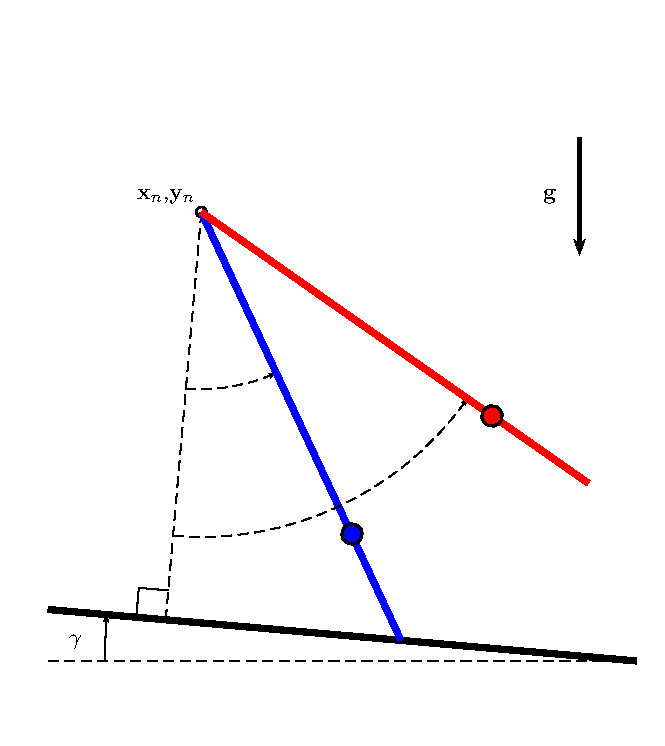
\includegraphics[width=0.7\textwidth]{CompassGait}
    \caption{Compass Gait}
    \label{fig:compassgait}
\end{center}
\end{figure}



\begin{figure}[!htbp]
  \begin{center}
      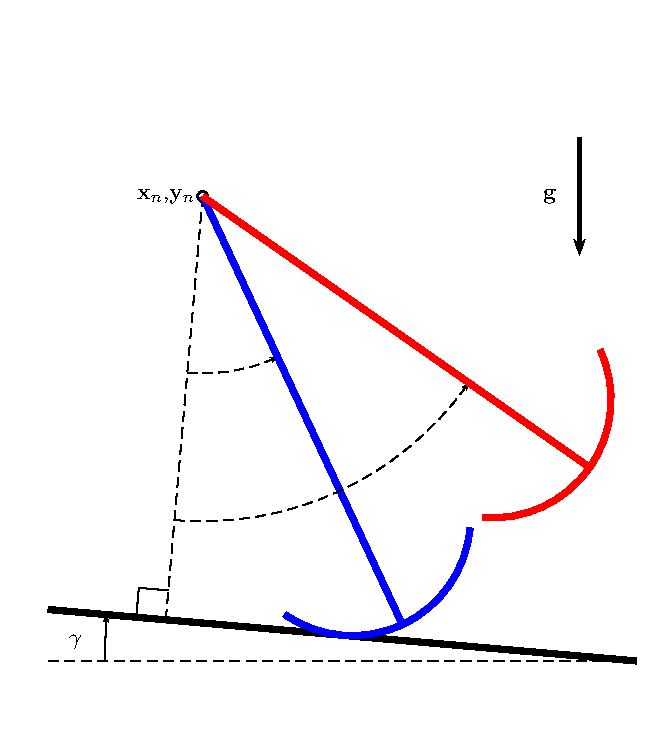
\includegraphics[width=0.7\textwidth]{CompassGaitArcFoot}
    \caption{Arc Foot Walker}
    \label{fig:arcfoot}
\end{center}
\end{figure}






Although the compass gait and arc foot model are different from  our walker with knee, the three models are all capable of passive walking and show limit cycles of similar shapes, as shown in Figure~\ref{fig:compassgaitlimitcycle} and Figure~\ref{fig:arcfootlimitcycle}.
\begin{figure}[!htbp]
  \begin{center}
      \includegraphics[width=0.7\textwidth]{compasGaitLimitCycle}
    \caption{the limit cycle of compass gait}
    \label{fig:compassgaitlimitcycle}
\end{center}
\end{figure}

\begin{figure}[!htbp]
  \begin{center}
      \includegraphics[width=0.7\textwidth]{arcfoot}
    \caption{the Limit Cycle of arcfoot}
    \label{fig:arcfootlimitcycle}
\end{center}
\end{figure}


This idea may be understood through the perturbation or averaging theory\citep{khalil2002nonlinear}.
Motions of some {\dof}s are relatively small, or have little effects on the topology.
From an alternative perspective, such motions are treated as perturbations.
For the knee walking example, the relatively small motion of knee is equivalent to perturbation of the leg length and the mass position.



Following this idea, feet are added to the original walker.
From experiment, the angle is almost rigid and the motion is relatively small.
From experience, foot will boost the stability.
Our hypothesis is that addition of the feet prolongs the double stance time, thus effort is applied to push the state towards the limit cycle.

This effects is modelled by the simplified liner model, as shown in Equation~\ref{eq:footheelstrike}.
\begin{equation}
\label{eq:footheelstrike}
\dot{q}_{st}=(1-r)\dot{q}_{st}+r\dot{q}^{desir}_{st}
\end{equation}
where the $\dot{q}_{st}$ is the state after the heel strike,
$r$ is the linear ration.
If foot action push the walker to normal perfectly, then $r=1$,
$\dot{q}^{desir}_{st}$ is the desired state, or the state on the limit cycle.


Adding feet will change the shape of limit cycle, which makes the original limit cycle more stable.
The gait is shown in Figure~\ref{fig:ToeGait}.
\begin{figure}[!htbp]
  \begin{center}
      \includegraphics[width=0.7\textwidth]{walkwithtoe}
    \caption{Walking with Toe}
    \label{fig:ToeGait}
\end{center}
\end{figure}


%And all the four system, can apply the same kind of symmetry group.

%as show in Figure.

%\begin{figure}[!htbp]
%  \begin{center}
%      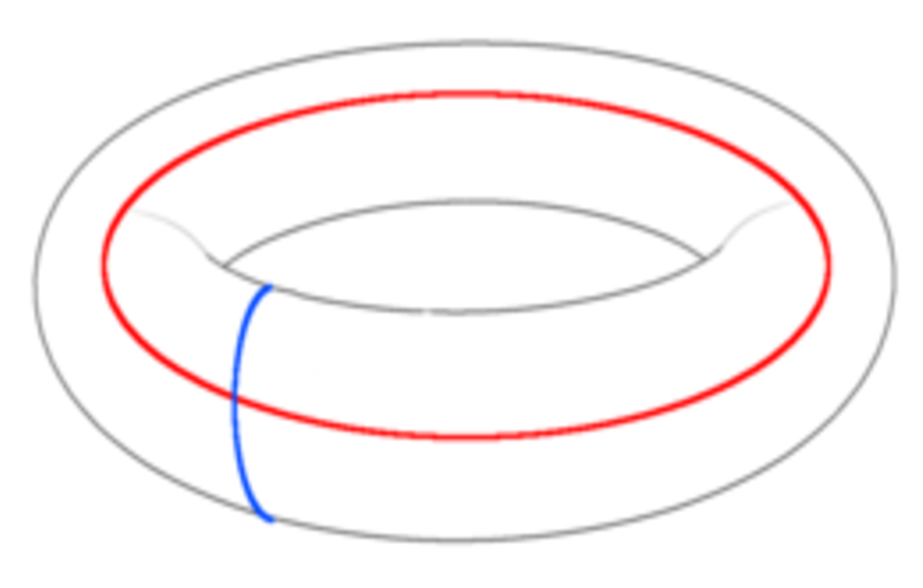
\includegraphics[width=0.7\textwidth]{Torus}
%    \caption{Approximate with Torus with a Circle}
%    \label{fig:approximate}  
%\end{center}
%\end{figure}


%Following this idea, although not implemented in this research, more dofs like foot may also possible.
%But that's just an extra level of complexity, without modifying the principles. 
\subsection{Symmetry Reduction}
For a dynamic system of high dimension, in some cases, the {\dof}s can be divided in a specific manner,
a lower dimensional dynamic system which captures the key properties of motion, 
and some extra {\dof}s that place the lower dimensional dynamics in higher dimensional space.
The extra {\dof}s have the same effects of group actions, and the dynamics can be controlled with lower dimensional model.



This idea helps to extend the 2D walker into 3 dimensions.
Rather than develop the full 3D dynamics, 3D walker are developed based on the 2D walker.
Motions in coronal plane and transverse plane transform sagittal plane dynamics.
The motion in Coronal Plane and Transverse Plane can be simplified as rigid body simulation, which place the 2D walker at a correct position in 3D space.

\subsubsection*{Lateral Motions}
An illustrative example shows the sway motions in the coronal plane.

\begin{figure}[!htbp]
  \begin{center}
      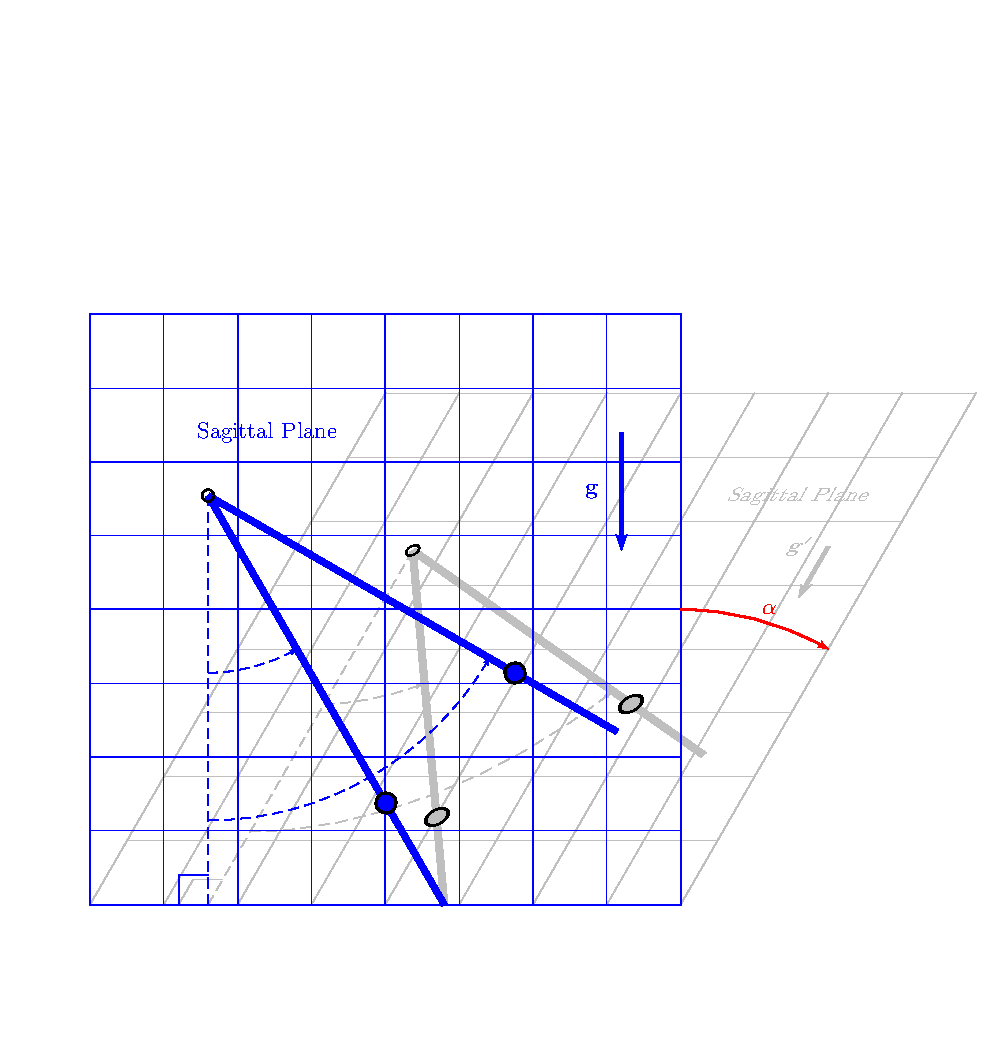
\includegraphics[width=0.7\textwidth]{sway3D}
    \caption{Sideway}
    \label{fig:sidesway}
\end{center}
\end{figure}

As shown in Figure~\ref{fig:sidesway}, the passive 2D walker walks on a terrain with a sway angle $\alpha$.
the gravity force on the spaghetti plane is decreased.
\[
\gv'=\cos(\alpha)\gv)
\]
where $\gv'$ is the projected gravity force on the spaghetti plane.
By substituting the projected gravity into the dynamic equations, we have
\begin{equation}
\label{eq:flyequation}
M(\mathbf{q}) \ddot{\mathbf{q}} + C(\mathbf{q,\qd})\dot{\mathbf{q}} + N'(\mathbf{q}) = 0
\end{equation}
The external force $N$ becomes $N'=cos(\alpha)N$

This has the same effect as applying speed action which the parameter $\ep$, where $\ep^2-1=\cos(\alpha)$.
The effects of sway motion on the 2D dynamics can be simulated by adjusting the speed action parameters $\ep$.
For walker with speed action controller, the effects of this {\dof} can be totally compensated.

The sway motion on the Coronal Plane is not passive based and unstable in nature\citep{kuo1999stabilization}.
Great effort is executed at the angle and waist for maintaining the posture.
Such motions are close relate to the character's motion purpose and not mainly governed by the natural dynamics, thus are left to the animators.
For procedure method, we can use \pd based method to make the walker sway about the center position.


\subsubsection*{Turning Motion}
Also the 2D dynamic model is free of the rotation on the transverse plane.
If the ground is rotating around the transverse plane at constant speed, the dynamics on the spaghetti plane will remain the same.
In three dimensions, the difference is that the centrifugal force is generated perpendicular to the sagittal plane, which is  compensated by the friction on the foot.

For the walker,  making a turning means rotate the spaghetti plane, this can be achieved by actuating the  hip joint of the supporting leg, as shown in Figure~\ref{fig:turn}.


\begin{figure}[!htbp]
  \begin{center}
      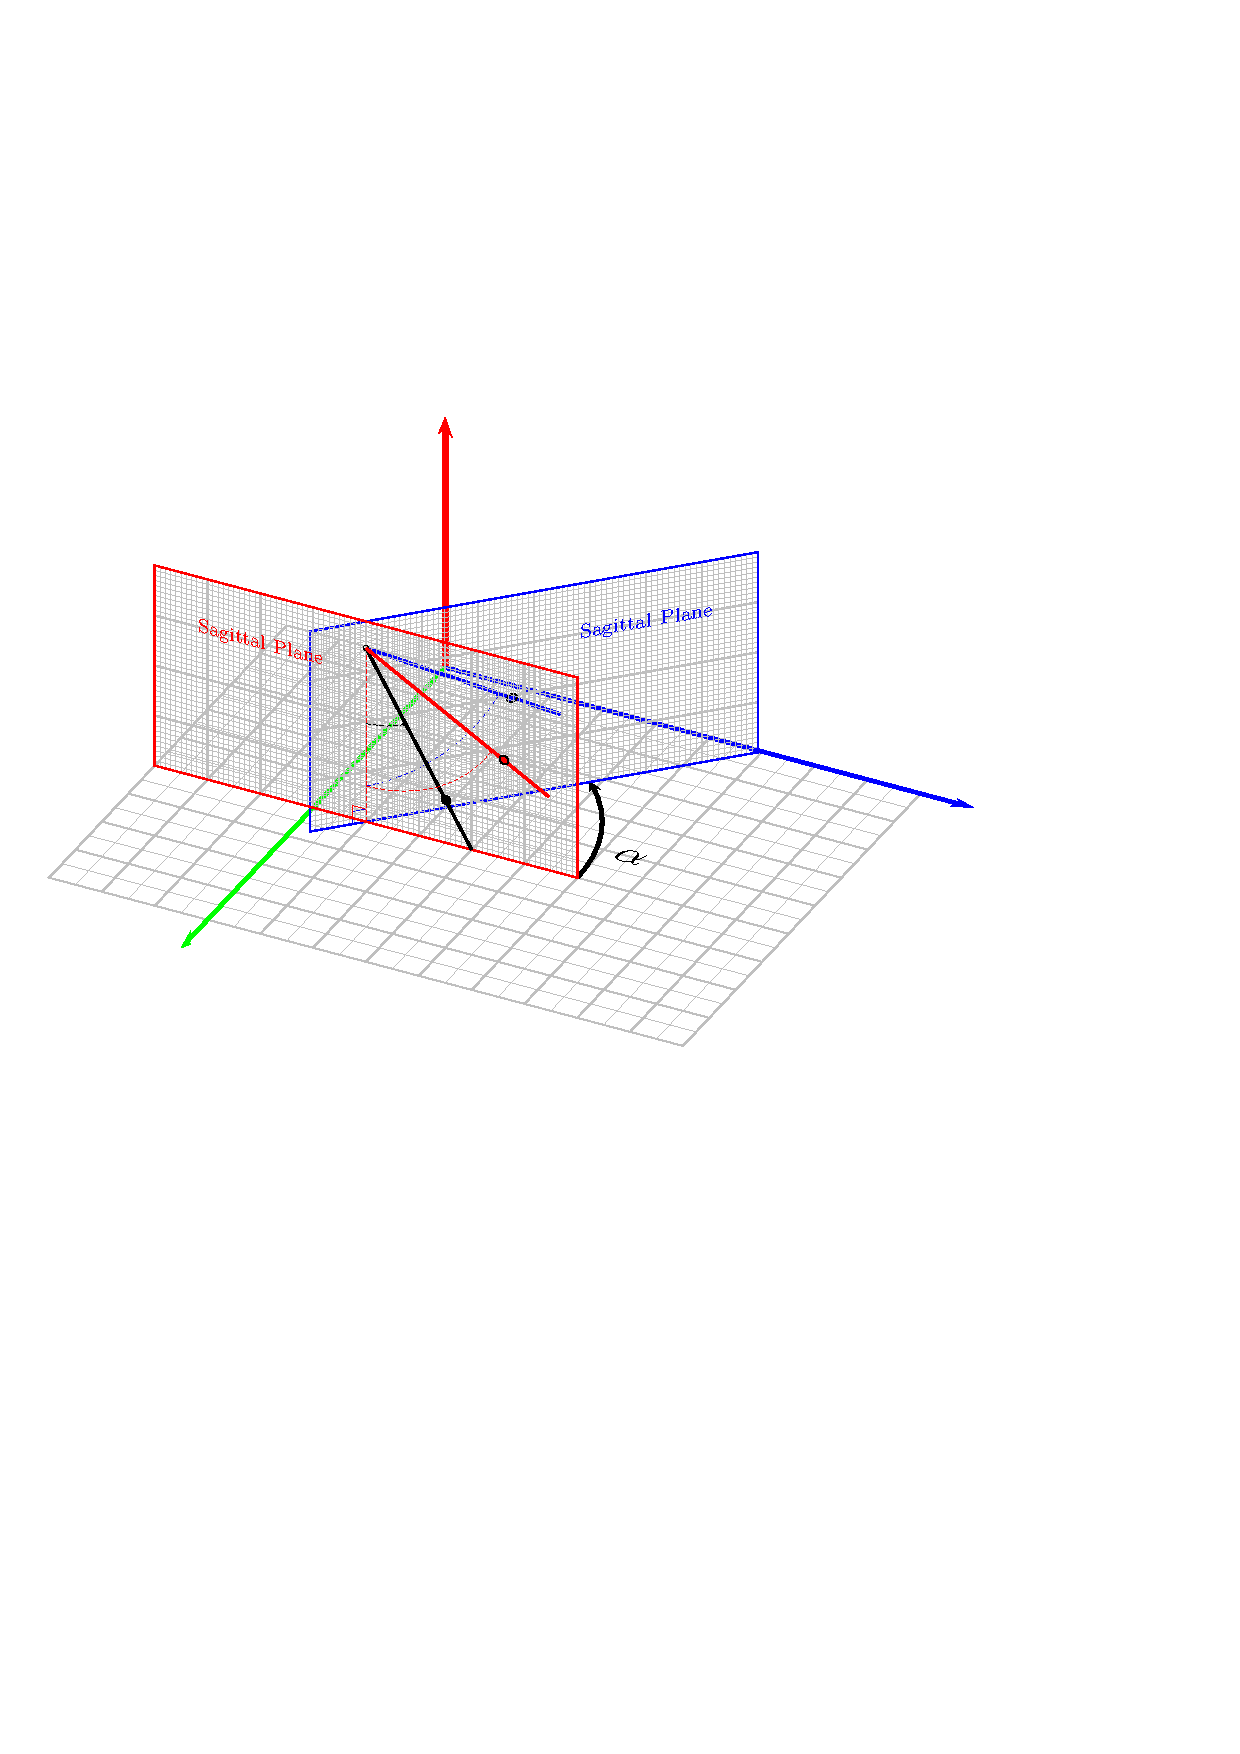
\includegraphics[width=0.7\textwidth]{Turn3d}
    \caption{Turn Actuation}
    \label{fig:turn}
\end{center}
\end{figure}


Same as the lateral motion, turning is not achieved by exploring the natural dynamics, but determined by the animator's purpose.
The animator determines the turning degree, and turning speed.
As a simplification, during the turning, the dynamic equations of 2D walker remain the same.





\begin{figure}[!htbp]
  \begin{center}
  $
     \begin{array}{ccccc}
\includegraphics[width=1in]{turn/0001.eps}&
\includegraphics[width=1in]{turn/0201.eps}&
\includegraphics[width=1in]{turn/0301.eps}&
\includegraphics[width=1in]{turn/0401.eps}&
\includegraphics[width=1in]{turn/0501.eps}
\\
\includegraphics[width=1in]{turn/0601.eps}&
\includegraphics[width=1in]{turn/0701.eps}&
\includegraphics[width=1in]{turn/0801.eps}&
\includegraphics[width=1in]{turn/0901.eps}&
\includegraphics[width=1in]{turn/1001.eps}
\\
\includegraphics[width=1in]{turn/1101.eps}&
\includegraphics[width=1in]{turn/1201.eps}&
\includegraphics[width=1in]{turn/1301.eps}&
\includegraphics[width=1in]{turn/1401.eps}&
\includegraphics[width=1in]{turn/1501.eps}
\\
\includegraphics[width=1in]{turn/1601.eps}&
\includegraphics[width=1in]{turn/1701.eps}&
\includegraphics[width=1in]{turn/1801.eps}&
\includegraphics[width=1in]{turn/1901.eps}&
\includegraphics[width=1in]{turn/2001.eps}
\\
\includegraphics[width=1in]{turn/2101.eps}&
\includegraphics[width=1in]{turn/2201.eps}&
\includegraphics[width=1in]{turn/2301.eps}&
\includegraphics[width=1in]{turn/2401.eps}&
\includegraphics[width=1in]{turn/2501.eps}

\end{array}$
    \caption{Walk And Turn}
    \label{fig:walkturn}
\end{center}
\end{figure}
Turning gaits are shown in ~\ref{fig:walkturn}




\section{Mechanical Coupling}
Many high {\dof}s systems have the tree topology, which is composed of many branches.
For such systems, the divide-and-conquer strategy can be applied to simplify the dynamic simulation difficulty.

The mechanical system can be treated as connecting many different simple components together.
Different components can be simulated independently, and the interactions between different parts form mechanical coupling.

If a mechanical system is in the following form
\[
\dot{\state}=F(\state)
\]
the state is $\state=[q_1,q_2,\qd_1,\qd_2]$
we can reform the the dynamic equation in the manner
$\state=[\state_1,\state_2]$
where
$\state_1=[q_1,\qd_1]$
$\state_2=[q_2,\qd_2]$

and the original system can be seen as two system coupled together
\begin{align}
\dot{\state}_1&=F_1(\state_1)+C_1(\state_1,\state_2)\nonumber\\
\dot{\state}_2&=F_2(\state_2)+C_2(\state_1,\state_2),\nonumber
\end{align}

if $C_{1,2} \ll F_{1,2}$, then the dynamic will be dominated by $F_{1,2}$ and $C_{1,2}$ can be treated as perturbations.
Controllers are designed according to $F_{1,2}$.

\subsection*{Branches Mechanical Structure}
In fact any mechanical system can be reformulated as entrainment network,
a proper division should separate the system at the places where the coupling is weak.
The weak coupling joints can be identified through the mechanical structure.
Usually, the joints where the system branches are a proper choice.

If the mechanical system is of  the structure shown in Figure~\ref{fig:brancefigure}.
\begin{figure}[!htbp]
  \begin{center}
      \includegraphics[width=0.5\textwidth]{multilink}
    \caption{brances mechanical structure}
    \label{fig:brancefigure}
\end{center}
\end{figure}

The  5 {\dof}s dynamic system is in the following form
\[
M\left[\begin{array}{c}
\ddot{q}_{1}\\
\ddot{q}_{2}\\
\ddot{q}_{3}\\
\ddot{q}_{4}\\
\ddot{q}_{5}\end{array}\right]+C\left[\begin{array}{c}
\dot{q}_{1}\\
\dot{q}_{2}\\
\dot{q}_{3}\\
\dot{q}_{4}\\
\dot{q}_{5}\end{array}\right]+\left[\begin{array}{c}
N_{1}(q_{1})\\
N_{2}(q_{2})\\
N_{3}(q_{3})\\
N_{4}(q_{4})\\
N_{5}(q_{5})\end{array}\right]=\left[\begin{array}{c}
u_{1}\\
u_{2}\\
u_{3}\\
u_{4}\\
u_{5}\end{array}\right]
\]

where $q_{1,2,3,4,5}$ are the configuration coordinates of $5$ links,
and the mass matrix is
\[
M=\left[\begin{array}{ccccc}
m_{11} & m_{12} & m_{13} & m_{14} & m_{15}\\
m_{12} & m_{22} & m_{23} & m_{24} & m_{25}\\
m_{13} & m_{23} & m_{33} & m_{34} & m_{35}\\
m_{14} & m_{24} & m_{34} & m_{44} & m_{45}\\
m_{15} & m_{25} & m_{35} & m_{45} & m_{55}\end{array}\right]
\]
and
\[
C=\left[\begin{array}{ccccc}
0 & c_{12}\dot{q_{2}} & c_{13}\dot{q}_{3} & c_{14}\dot{q}_{4} & c_{15}\dot{q}_{5}\\
-c_{12}\dot{q_{1}} & 0 & c_{23}\dot{q}_{3} & c_{24}\dot{q}_{4} & c_{25}\dot{q}_{5}\\
-c_{13}\dot{q_{1}} & -c_{23}\dot{q}_{2} & 0 & c_{34}\dot{q}_{4} & c_{35}\dot{q}_{5}\\
-c_{14}\dot{q_{1}} & -c_{24}\dot{q}_{2} & -c_{34}\dot{q}_{3} & 0 & c_{45}\dot{q}_{5}\\
-c_{15}\dot{q_{1}} & -c_{25}\dot{q}_{2} & -c_{35}\dot{q}_{3} & -c_{45}\dot{q}_{4} & 0\end{array}\right]
\]





For the branch structure in Figure \ref{fig:brancefigure},
the coefficient of unconnected links will be zero, thus
\[
M=\left[\begin{array}{ccccc}
m_{11} & m_{12} & m_{13} & m_{14} & m_{15}\\
m_{12} & m_{22} & m_{23} & 0 & 0\\
m_{13} & m_{23} & m_{33} & 0 & 0\\
m_{14} & 0 & 0 & m_{44} & m_{45}\\
m_{15} & 0 & 0 & m_{45} & m_{55}\end{array}\right]
\]

and
\[
C=\left[\begin{array}{ccccc}
0 & c_{12}\dot{q_{2}} & c_{13}\dot{q}_{3} & c_{14}\dot{q}_{4} & c_{15}\dot{q}_{5}\\
-c_{12}\dot{q_{1}} & 0 & c_{23}\dot{q}_{3} & 0 & 0\\
-c_{13}\dot{q_{1}} & -c_{23}\dot{q}_{2} & 0 & 0 & 0\\
-c_{14}\dot{q_{1}} & 0 & 0 & 0 & c_{45}\dot{q}_{5}\\
-c_{15}\dot{q_{1}} & 0 & 0 & -c_{45}\dot{q}_{4} & 0\end{array}\right]
\]








This matrix of dynamic equation can be grouped in the following manner:
where
\[
M=\left[\begin{array}{ccc|cc}
m_{11} & m_{12} & m_{13} & m_{14} & m_{15}\\
m_{12} & m_{22} & m_{23} & 0 & 0\\
m_{13} & m_{23} & m_{33} & 0 & 0\\ \hline
m_{14} & 0 & 0 & m_{44} & m_{45}\\
m_{15} & 0 & 0 & m_{45} & m_{55}\end{array}\right]
=\left[\begin{array}{cc}
M_{33} & M_{c32}\\
M_{c32} & M_{22}\end{array}\right]
\]

and
\[
C=
\left[\begin{array}{ccc|cc}
0 & c_{12}\dot{q_{2}} & c_{13}\dot{q}_{3} & c_{14}\dot{q}_{4} & c_{15}\dot{q}_{5}\\
-c_{12}\dot{q_{1}} & 0 & c_{23}\dot{q}_{3} & 0 & 0\\
-c_{13}\dot{q_{1}} & -c_{23}\dot{q}_{2} & 0 & 0 & 0\\ \hline
-c_{14}\dot{q_{1}} & 0 & 0 & 0 & c_{45}\dot{q}_{5}\\
-c_{15}\dot{q_{1}} & 0 & 0 & -c_{45}\dot{q}_{4} & 0\end{array}\right]
=\left[\begin{array}{cc}
C_{33} & C_{c32}\\
C_{c32} & C_{22}\end{array}\right]
\]

The coupling network of two dynamic equations is
\[
M_{33}\left[\begin{array}{c}
\ddot{q}_{1}\\
\ddot{q}_{2}\\
\ddot{q}_{3}\end{array}\right]+C_{33}\left[\begin{array}{c}
\dot{q}_{1}\\
\dot{q}_{2}\\
\dot{q}_{3}\end{array}\right]+\left[\begin{array}{c}
N_{1}(q_{1})\\
N_{2}(q_{2})\\
N_{3}(q_{3})\end{array}\right]=\left[\begin{array}{c}
u_{1}\\
u_{2}\\
u_{3}\end{array}\right]-\left[\begin{array}{c}
m_{14}\ddot{q}_{4}+m_{15}\ddot{q}_{5}\\
0\\
0\end{array}\right]-\left[\begin{array}{c}
c_{14}\dot{q}_{4}^{2}+c_{15}\dot{q}_{5}^{2}\\
0\\
0\end{array}\right]
\]

\[
M_{22}\left[\begin{array}{c}
\ddot{q}_{4}\\
\ddot{q}_{5}\end{array}\right]+C_{22}\left[\begin{array}{c}
\dot{q}_{4}\\
\dot{q}_{5}\end{array}\right]+\left[\begin{array}{c}
N_{4}(q_{4})\\
N_{5}(q_{5})\end{array}\right]=\left[\begin{array}{c}
u_{1}\\
u_{2}\end{array}\right]-\left[\begin{array}{c}
m_{14}\\
m_{15}\end{array}\right]\ddot{q}_{1}-\left[\begin{array}{c}
-c_{14}\\
-c_{15}\end{array}\right]\dot{q}_{1}^{2}
\]

From mechanical perspective, this is equivalent to simulating two branches of the mechanical structure independently and coupling is treated as perturbation effects.
Figure \ref{fig:mechcouple} shows how the mechanical structure is decoupled.
\begin{figure}[!htbp]
  \begin{center}
      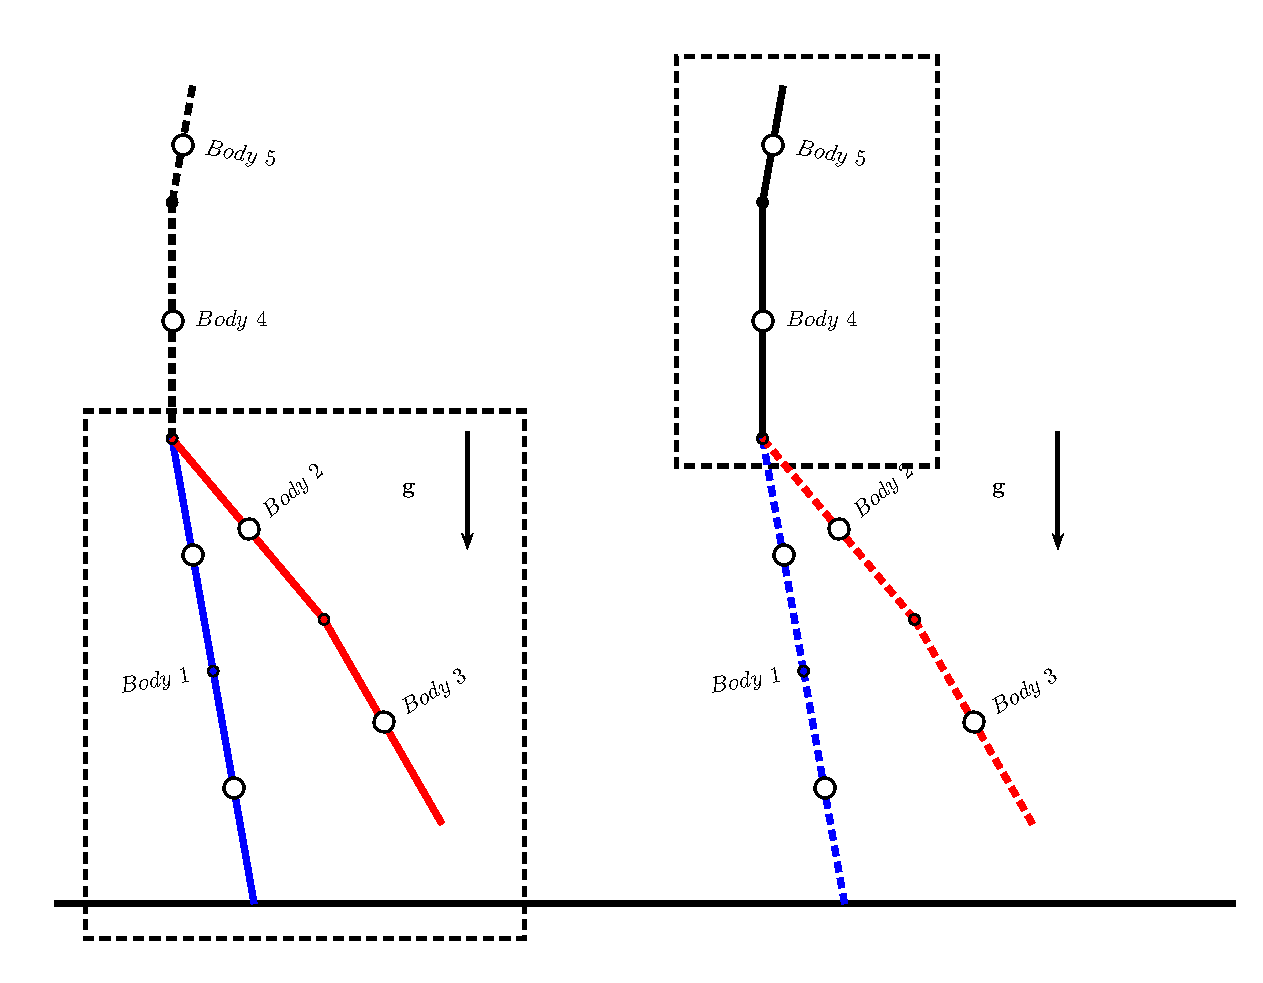
\includegraphics[width=0.7\textwidth]{multilinkCoupled}
    \caption{mechanical coupling}
    \label{fig:mechcouple}
\end{center}
\end{figure}








\subsection{Torso And Arm}
Using this mechanical coupling idea, the arm and torso motions are incorporated in our simulation.
Three variables are added for the torso, the angle is $q_{tor}$,  mass $m_{tor}$ and the distance from the hip is $l_{tor}$.
With upper body, the equation for walking becomes
\begin{equation}
\label{eq:walkcouplewithtorso}
M\ddot{q}+C\dot{q}+N=u-\left[\begin{array}{c}
m_{tor}l_{tor}Lcos(q_{1}-q_{tor})\ddot{q}_{tor}\\
0\\
0\end{array}\right]-\left[\begin{array}{c}
m_{tor}l_{tor}L\sin(q_{1}-q_{tor})\dot{q}_{tor}^{2}\\
0\\
0\end{array}\right]
\end{equation}

From the Equation~\ref{eq:walkcouplewithtorso}, if the torso is kept still, lower body walking will not be effected.
In real life walking, the upper body usually keeps straight upward, the coupling input from the upper body is very small.



The dynamic of the torso can be modelled as an inverted pendulum perturbed by lower body dynamic, as follows.
\begin{equation}
\label{eq:torsodynamic}
m_{tor}l_{tor}^{2}\ddot{q}_{tor}=gm_{tor}l_{tor}sin(q_{tor})-(m_{tor}l_{tor}Lcos(q_{1}-q_{tor})\ddot{q}_{1}-m_{tor}l_{tor}Lsin(q_{1}-q_{tor})\dot{q}_{1}^{2})
\end{equation}

by analysing the Equation~\ref{eq:torsodynamic},  torso motion is unstable in nature,  control effort must be exerted to maintain its posture.
Such control task is trivial, simple \pd controller will work for maintaining stability, but the resulting swaying may not be natural looking..

The control method adopted by this research is based on the controlled Lagrange method.
Although inverted pendulum is not stable, pendulum is stable.
Through shaping the potential energy by control effort, we  rotate the inverted pendulum to make it a pendulum.

When the stable pendulum is coupled with the walking motion, stable entrainment happens, so the torso and walking motion coordinate naturally. 
Figure ~\ref{fig:torsolegentrainment} shows the entrainment of the torso motion and walking, the body sway and walking synchronized.
\begin{figure}[!htbp]
  \begin{center}
      \includegraphics[width=0.5\textwidth]{torsoAndLeg}
    \caption{The Mechanical Entrainment of Leg And Torso}
    \label{fig:torsolegentrainment}
\end{center}
\end{figure}




Note that in real-life, torso is closely related to motion purpose and not governed by natural dynamic properties.
For animation application purpose,  it is unnecessary to control the upper body dynamically.
We can use procedure or other ``IK'' method to generate primary  motion of the upper body, walking dynamics perturbations are added for secondary motions.
The motion of arms can be incorporated by following the same principles, it is just another level of complexity.


\section{Time Shift}

For reptile and fish, the main challenge rests in synthesizing the flexible vertebrate which is composed of many {\dof}s.
Such {\dof}s are similar and equally important, it is not proper to reduce any \dof through symmetry or mechanical coupling.

For such mechanical structures, an ad-hoc method is proposed, each controller controls just one joint.
The hypothesis that since the joints are similar, their dynamics and motion should also be similar.
Thus the same control strategy is applied for every joint.
Motions of each joints are differentiate by the group action.


The idea can also be applied for boid system\citep{reynolds1987flocks}.
Compared with traditional boid method, the new method will make the boid system stable and easy to control.
Traditional Rule based boid system does not grantee stability, and sometime result in unexpected results.
Based on the method of \moit, if all the agent motions are based on the same attractor, ,
The uniformity of final motions of agents is a grantee.
The differences  among the agents are modelled by different group actions.

\subsection*{Fish Swimming}
These ideas are applied to synthesis of the fish swimming motion.
In this application,the group action is the Time Shift.
The fish is made up 8 links, and each {\dof} is controlled by a neural oscillator.
The $8$ \cpg have the same parameters, but have different initial positions. 
Thus they have the same limit cycle, but different phases, as shown in Figure~\ref{fig:fishplot}



\begin{figure}[!htbp]
  \begin{center}
      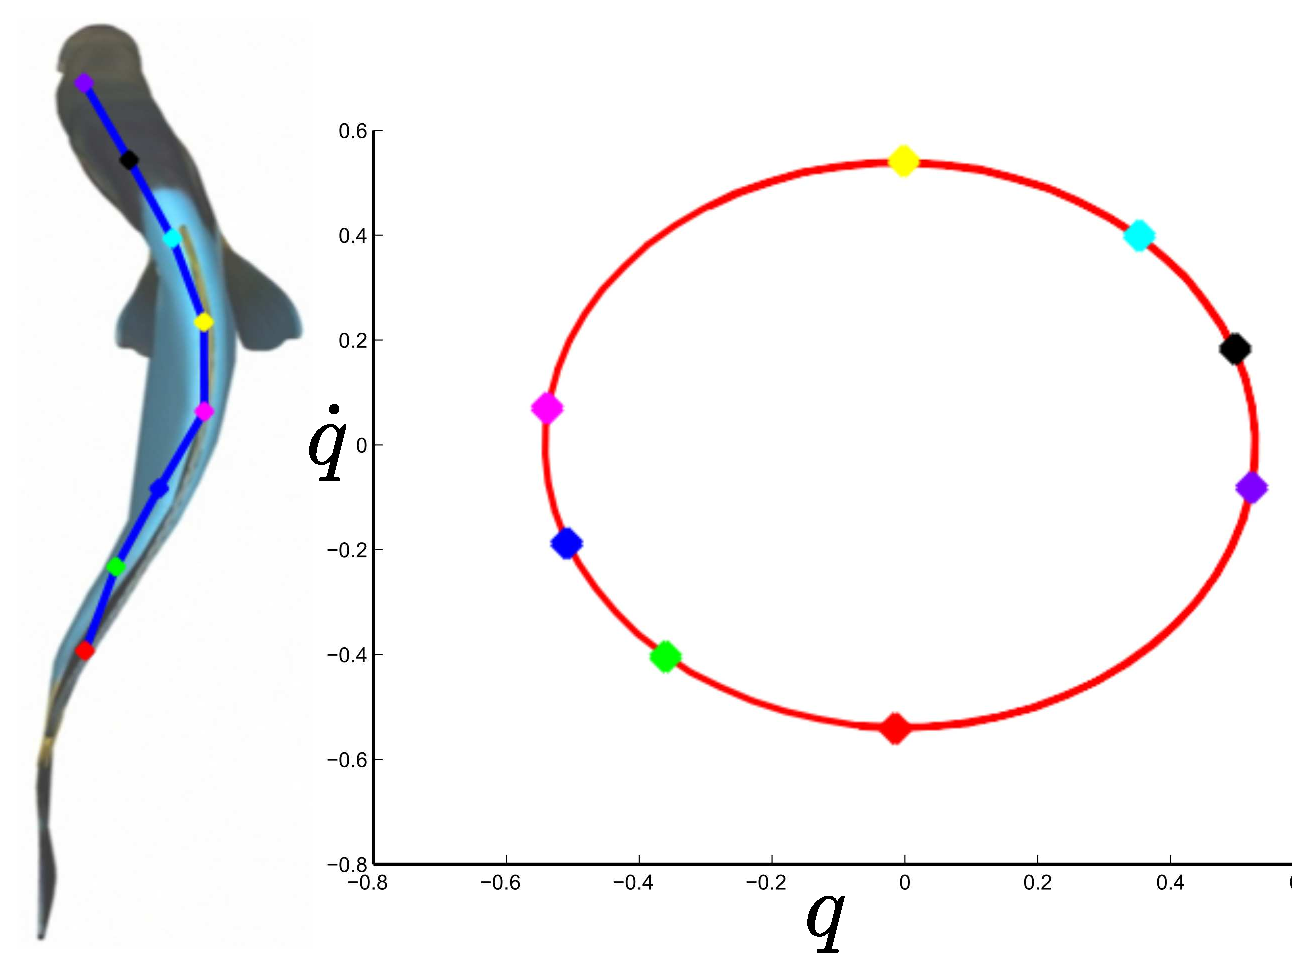
\includegraphics[width=0.5\textwidth]{fish_plot}
    \caption{CPG for Fish}
    \label{fig:fishplot}
\end{center}
\end{figure}




Simplified dynamic model is used.
Each joint is modelled as a spring system, as Equation~\ref{eq:fishdynamics}
\begin{equation}
\label{eq:fishdynamics}
\ddot{q}=Kq
\end{equation}
where $q$ is the joint angle.
A simple fluid dynamic model is adopted,  swimming speed is propotional to the square of the vibrating velocity.
And Figure~\ref{} shows the gait of a fish swimming in line.
\begin{figure}[!htbp]
  \begin{center}
      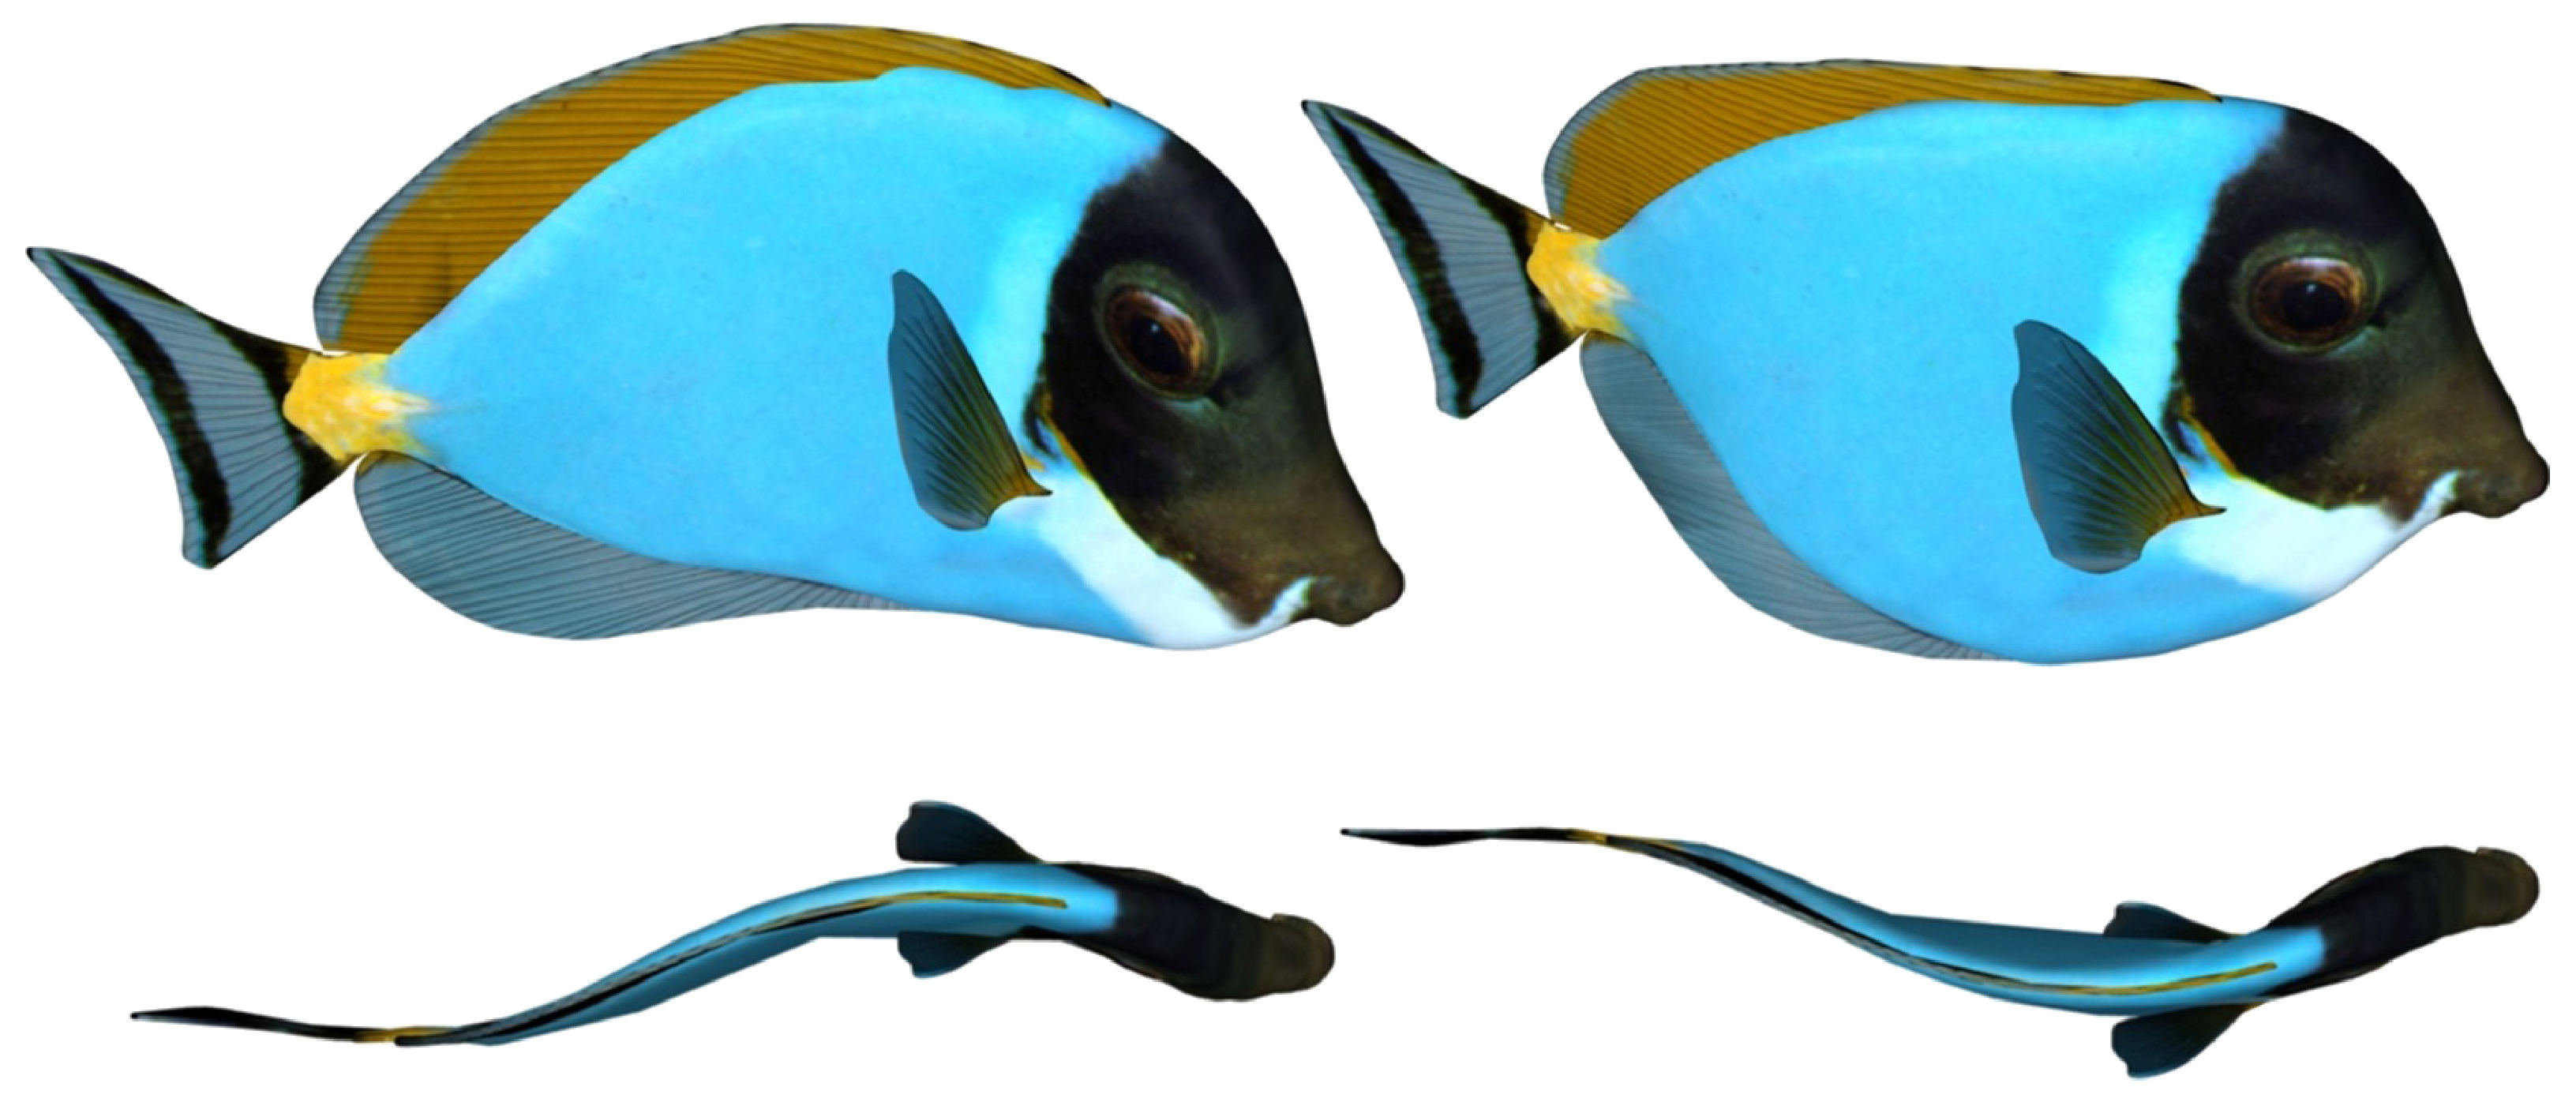
\includegraphics[width=0.5\textwidth]{fish_swimming}
    \caption{Swimming Motion by our method}
    \label{fig:fishswimming}
\end{center}
\end{figure}


\subsection{Swimming Motion Tweaking}

There are lots of group actions available for tweaking the fish swimming motion.
Offset Action will result in the fish turning,
Speed Action will make the fish swim more fast.
Energy Action will modify the swimming intensity.
When a group action is chosen, the action is applied on all the {\dof}s.


Figure~\ref{fig:fishswimline} shows the swimming gaits in a line.
Figure~\ref{fig:fishswimturn} show the the turning gait.


\begin{figure}[!htbp]
\begin{center}
      \includegraphics[width=\textwidth]{SwimLine}
    \caption{Fish Swim}
    \label{fig:fishswimline}
\end{center}
\end{figure}


\begin{figure}[!htbp]
\begin{center}
      \includegraphics[width=\textwidth]{SwimTurn}
    \caption{Fish Swim Turn}
    \label{fig:fishswimturn}
\end{center}
\end{figure}









